\documentclass{article}

\usepackage[utf8]{inputenc}
\usepackage{ngerman}

\usepackage{graphicx}
\usepackage{subfigure}

\usepackage{lipsum}
\usepackage{pdfpages}

\usepackage{color}
\usepackage{verbatim}

\usepackage{varioref}
	\labelformat{figure}{Abbildung~#1}


\begin{document}
%opening

%\includepdf{Titlepage}

\newpage

\tableofcontents

\newpage
	
\section{Einleitung}

\vspace{2cm}
\subsection{Spielprinzip}

\vspace{2cm}
\subsection{Zielsetzung}

\vspace{2cm}
\subsection{Projektumfeld}


\newpage
\section{Projektplanung \textcolor{red}{(in Arbeit - Chris )}}


\vspace{2cm}
\subsection{Projektphasen  \textcolor{red}{(in Arbeit - Chris )}}

\vspace{2cm}
\subsection{Ressourcenplanung  \textcolor{red}{(in Arbeit - Chris )}}

\vspace{2cm}
\subsection{Entwicklungsprozess  \textcolor{red}{(in Arbeit - Chris )}}

\newpage
\section{Das Spiel}

\vspace{2cm}
\subsection{Hauptmenü \textcolor{blue}{(QA - Lars )}}

Das Hauptmenü stellt den Einstieg in unser Spiel dar. Hier wird der Spieler empfangen.

\vspace{1cm}
\subsubsection{Spiel Starten \textcolor{blue}{(QA - Lars )}}

Durch das Betätigen des Buttons „Starten“ gelangt man in den Ingame-Bereich. Bevor es mit dem Spielen losgeht, öffnet sich am Anfang jedes
Levels ein kleiner Tutorialbildschirm, welcher auch als Pause für den Spieler gedacht ist. Weiterhin kann er hier kurz verweilen um sich vorzubereiten
und so die Konzentration zu steigern.

\vspace{1cm}
\subsubsection{Einstellungen \textcolor{blue}{(QA - Lars )}}

Mit den Settings kann man seine persönlichen Einstellungen an dem Spiel vornehmen. Es lassen sich der Schwierigkeitsgrad und die Musiklautstärke
ändern. Auch gibt es hier eine ausführliche Beschreibung der Steuerung.

\vspace{1cm}
\subsubsection{Statistiken \textcolor{blue}{(QA - Lars )}}

Unter Statistics lässt sich der Spielfortschritt in den einzelnen Leveln begutachten. So findet man eine detaillierte Auflistung von Timeboni, eingesammelten
Münzen und den Score für jedes Level. Des Weiteren werden auch die gesamte Todeszahl und der Totalscore erfasst. Nach Beenden des Spiels wird die Statistik gelöscht. Die Statistik wird zu dem  nur zu einem Run aufgestellt, sobald der Spieler das Spiel durchgespielt hat und einen neuen Run startet wird die alte Statistik gelöscht.

\begin{figure}
	\centering
	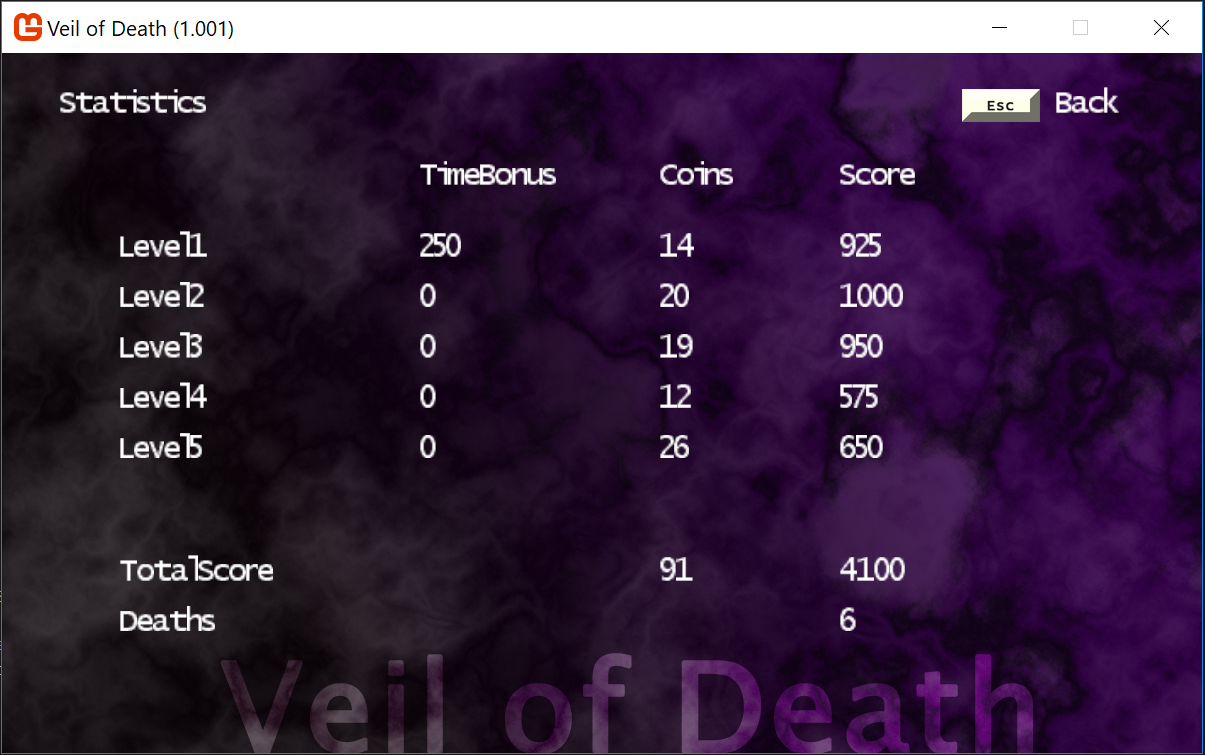
\includegraphics[width=1\textwidth]{Statistics}
	\caption{Statistik
		\label{fig:statistics}}
\end{figure}

\vspace{1cm}
\subsubsection{Credits \textcolor{blue}{(QA - Lars )}}

Diese Option gibt Auskunft über die Konstellation des Teams und die jeweiligen Aufgabenbereiche.

\vspace{1cm}
\subsubsection{Sonstiges}

\vspace{2cm}
\subsection{Spielwelt}

\vspace{1cm}
\subsubsection{Levelgenerator  \textcolor{red}{(in Arbeit - Chris )}}

\vspace{1cm}
\subsubsection{Player}

\vspace{1cm}
\subsubsection{Fallen \textcolor{blue}{(QA - Lars )}}

In unserem Spiel finden zwei Arten von Fallen Verwendung. Es gibt Fallen, die den Spieler verlangsamen. Weiterhin haben wir eine
weitere Art Fallen, die zum plötzlichen Tod führen. Dieser wird durch die Kollision mit den Fallen ausgelöst. Der Tod wird durch die
Spiketrap und die Spikeroll verursacht. Außerdem ist zu erwähnen, dass die Spikeroll beweglich ist. Je nach Schwierigkeitsgrad nimmt
die Bewegungsgeschwindigkeit dieser zu. Bei der Slowtrap wird der Spieler für eine bestimmte Dauer verlangsamt. Nach dem der Spieler
mehrere Male durch die Slowtrap gelaufen ist, wird er letztendlich vom Veil eingeholt und stirbt. Dadurch haben wir verschiedene Faktoren,
die das Spiel zusätzlich erschweren sollen.

\vspace{1cm}
\subsubsection{Feedback}

\vspace{1cm}
\subsubsection{Assets}

\newpage
\section{Technische Umsetzung}

\vspace{2cm}
\subsection{Codestruktur}
\textcolor{green}{- siehe TDD}

\vspace{1cm}
\subsubsection{GameStates}
\textcolor{green}{- alle mal kurz anreißen}

\vspace{1cm}
\subsubsection{Globale Klassen \textcolor{blue}{(QA - Lars )}}
%\textcolor{green}{- GameConstants \newline
%- Gamemanager (siehe TDD)}

In der GameConstants-Klasse wurden alle static-Objekte des Projektes angelegt. Hier zu gehören Variablen die klassenübergreifend gebraucht werden.
Weiterhin sind hier alle wichtigen Soundeffekte hinterlegt. Eine Kamerainstanz ist auch hinterlegt. Des Weiteren sind auch wichtige Angaben zum Sprung
hier hinterlegt, wie die Sprungweite und Sprunghöhe. Der Vorteil dieser Klasse ist, dass hier alle Zahlenwerte gebündelt gesammelt wurden, die global im
Projekt verwendet werden. Dadurch sind Änderungen sehr schnell vornehmbar.

Der GameManager ist ein Singelton-Pattern in dem das Spiels verwaltet wird und bildet somit das Herz des Spiels. Durch unsere Mapgeneration auf die wir
vorhin eingegangen sind, ist es notwendig zu wissen, welche Fallen aktiv sind und welche nicht. Dafür werden die Fallen in ihren Listen gespeichert, welche
immer aktualisiert werden, durch hinzufügen oder löschen der Fallen. So gibt es für jede Fallenart eine Liste. Das gleiche Prinzip gilt auch für die Münzen.
Der Todesschleier wird von hier aus gesteuert. Levelverwaltung, Scorehandhabung und das Speichern der Statistik sind ein weiterer Bestandteil des GameManagers.

\vspace{2cm}
\subsection{InGame}

\vspace{1cm}
\subsubsection{Movement \textcolor{blue}{(QA/ Grafik fehlt - Lars )}}
%\textcolor{green}{- Lane prinzip \newline
%- Jump-Funktion (Parabel anhand von Geschwindigkeit)}

Unser Spielercharakter kann sich auf drei Arten fortbewegen. Er kann Rennen, Sliden und Springen. Der Sprung wurde an eine
Wurfparabel angepasst, sodass sich der Sprung wie ein Wurf verhält. Der Spielercharakter gewinnt an Höhe bis er den Scheitelpunkt
erreicht und sinkt danach wieder zu Boden. Dadurch ist der Sprung symmetrisch, sowohl die Anstiegs- und Abstiegskurve sind gleich.

%Grafik Wurfparabel einfügen

Durch das Laneprinzip unseres Spiels haben wir uns gegen einen flüssigen Übergang des Spielercharakters beim Wechseln der Lanes
entschieden. Wir lassen ihn wirklich zwischen den Lanes switchen, so dass er sich nicht in Zwischenbereichen aufhalten kann.

\vspace{1cm}
\subsubsection{Collision \textcolor{blue}{(QA - Lars )}}

\begin{comment}
\textcolor{green}{2 Arten: \newline
- AABB für Spiketrap und spikeroll \newline
- Gridposition für Coins und Slowtrap}
\end{comment}

In unserem Spiel haben wir zwei unterschiedliche Kollisionmethoden verwendet.
Zum Einen Arbeiten wir mit Gridpositions für statische Objekte und mit den
Axis-Alligned-Bounding-Boxes für bewegbare Objekte.\newline
\newline
Gridpositions eignen sich hervorragend für statische Objekte in Spielen, daher werden die Kollisionen
von Münzen und Slowtraps von ihnen verwaltet. Hier für werden die Positionen von unseren kollidirbaren
Objekten abgespeichert. Die Kollision wird dann mit Hilfe von if-Bedingungen berechnet.\newline
\newline
Axis-Alligned-Bounding-Boxes berechnen für uns die Kollisionen mit beweglichen Obejkten, so dass jedes Objekt seine eigene
Bounding Box hat. Hier für wird um das Objekt eine Hülle gespannt. In unserem Spiel haben wir die jeweiligen Maximalwerte
der Modelle in Betrachtung der Achsen gewählt. Die Kollision entsteht wenn die Minimalwerte der Achsen von Körper A kleiner
als die Maximalwerte von Körper B sind. Sowie die Maximalwerte der Achsen von Körper A größer sind als die Minimalwerte der
Achsen von Körper B. Anders gesagt wenn die erweiterte konvexe Hülle des einen Körpers, die des Anderen schneidet.

%Grafik einfügen



\vspace{1cm}
\subsubsection{Sontiges}

\vspace{2cm}
\subsection{GUI}

\vspace{1cm}
\subsubsection{Panel System \textcolor{red}{(in Arbeit - Chris)}}

\vspace{2cm}
\subsection{Rendering}

\vspace{1cm}
\subsubsection{Aufbau}

\vspace{1cm}
\subsubsection{Weltkoordinaten \textcolor{blue}{(QA - Lars )}}

Der Up-Vektor in unserem Spiel ist nicht wie üblich die y-Achse sondern die z-Achse. Weiterhin bildet der Koordinatenursprung am 
Anfang nicht die Mitte unserer Lanes, er liegt am linken Rand. Darauf aufbauend wird die Spielwelt mit Hilfe unserer Blocksize generiert. Hierfür 
werden lediglich die x- und y-Achse benötigt. Die z-Achse wird für die Kollisionsberechnung benötigt. Die Kamera befindet sich am Anfang 
vor unserer eigentlich Spielwelt, um die gewünschte Perspektive zu erzeugen. Im weiteren Verlauf des Spiels verfolgt sie dann den Spieler
auf einer Linie entlang der y-Achse mit konstanter Geschwindigkeit. Die Kamera wurde somit aus dem Koordinatenursprung zu ihrem letztendlichen
Platz verschoben. Somit bildet die Weltmatrix diese Translation ab. Eine genaue Darstellung können sie \ref{fig:coordinates} entnehmen.

\begin{figure}
	\centering
	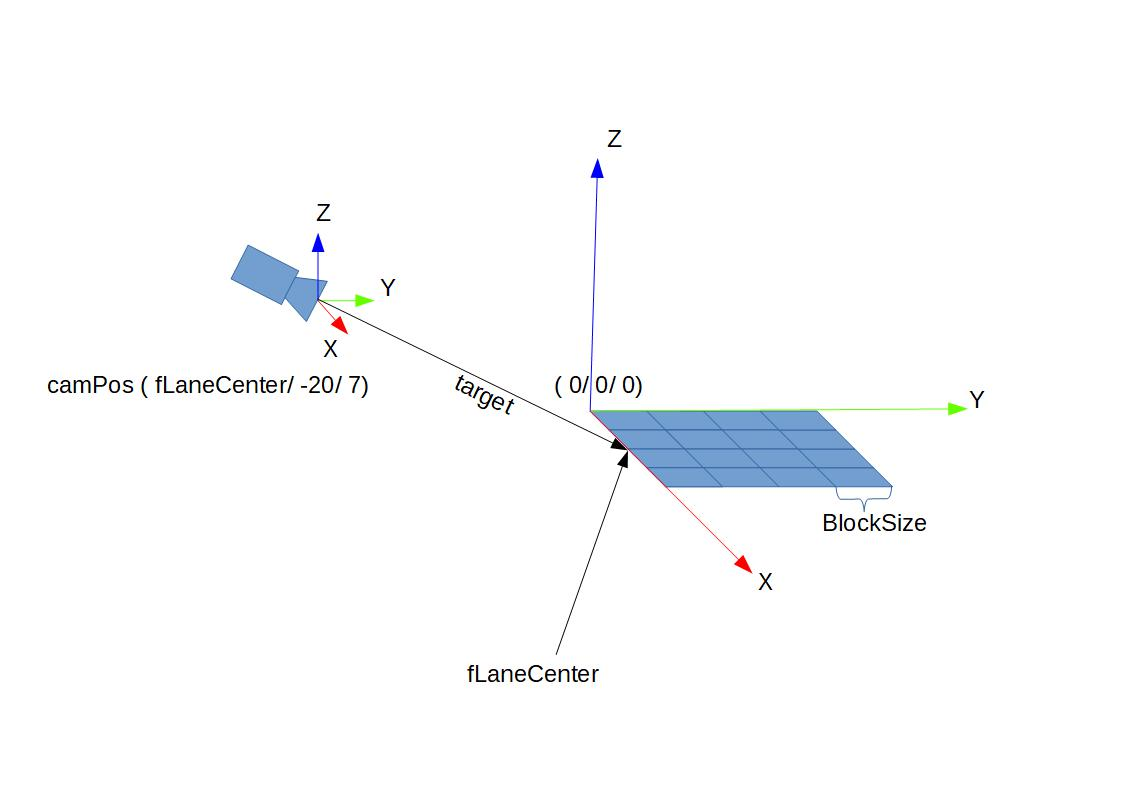
\includegraphics[width=1\textwidth]{Weltkoordinaten}
	\caption{Weltkoordinaten
		\label{fig:coordinates}}
\end{figure}

\vspace{1cm}
\subsubsection{Animation \textcolor{blue}{(QA - Lars )}}
Die Animation der Modelle erfolgt unter den Gebrauch einer Bibliothek. Hierfür benötigt man eine .x-Datei.
Des Weiteren wird eine Textdatei benötigt, in der festgehalten ist, wie das Modell animiert werden soll.
In dieser Textdatei kann man auf das jeweilige Modell bezogen so viele Methoden (Animationparts) erstellen
wie man möchte. Man kann entscheiden, ob die Animation wiederholt werden soll oder einfach gespielt wird.
Außerdem wird hier das Start- und Endframe der Animation festgelegt. Auch die Animationsdauer ist eine weitere
Einstellungsoption. Nach dem man die jeweiligen Einstellungen für seine Methoden festgelegt hat, kann man diese
im späteren Code unter ihrem angegebenen Namen aufrufen. Bevor man diese jedoch aufrufen kann, muss die
Textdatei gelesen werden. Es gilt weiterhin zu beachten, dass nur eine Animations gleichzeitig abgespielt werden kann.
Darunter ist zu verstehen, dass es nicht möglich ist die Animation in mehrere Schichten aufzuteilen, sodass es möglich ist
mehrere Animationen abzuspielen aber nur Eine sichtbar zu zeichnen, während die Anderen im Hintergrund weiterlaufen.
Diese Option würde den Übergang zwischen unterschiedlichen Animationen vereinfachen, da man die Zweite einfach auf
transparent stellen würde.

\vspace{1cm}
\subsubsection{Partikel Effekte}

\vspace{2cm}
\subsection{Statistik}


\newpage
\section{Projektverlauf}

\vspace{2cm}
\subsection{Prototypen}

\vspace{1cm}
\subsubsection{Prototyp 1 - Alexander Heck und Robert Jendersie}

\vspace{1cm}
\subsubsection{Prototyp 2 - Christoph Dollase und ???}

\vspace{1cm}
\subsubsection{Prototyp 3 - Lars Wagner und Mattis Hagen \textcolor{blue}{(QA - Lars )}}
Unser Prototyp war ein Spaceshooter indem man ein Raumschiff steuern konnte, welches Meteoriten ausweichen musste.
Es ist auch möglich gewesen die Meteoriten abzuschießen. Für den Abschuss der Meteoriten hat man Punkte gekriegt. Das Spiel endet sobald das Raumschiff keine Trefferpunkte mehr hat, welche man verliert wenn man mit den Meteoriten kollidiert. Ziel des Spiels ist es solange wie möglich zu überleben und seinen Highscore zu maximieren.

\noindent Das Spiel basiert auf einem Grid-System, da die Meteoriten nur in einem Grid aus festgelegten Punkten spawnen können. Die Kamera ist starr fixiert und lässt sich nur zu Debugzwecken bewegen. Die Meteoriten rotieren um eine zufällig gewählte Achse während sie sich dem Spieler nähern. Mit der Zeit nimmt die Geschwindigkeit der Meteoriten zu.
Unsere Laserstrahlen sind Punkte die wir dann als separate von einander getrennte Linien zeichnen lassen.
Auch wurde der Spieler über die GUI über seinen Score, seine verbliebenen Trefferpunkte informiert.
Die Asteroiden werden durch den MeteorHandler verwaltet. Dadurch sind nie mehr als 20 Meteoriten auf dem Bildschirm, sobald ein Meteor hinter der Kamera despawnte, spawnte sofort ein Neuer.

\vspace{2cm}
\subsection{Meilensteine}

\vspace{1cm}
\subsubsection{MS I}

\vspace{1cm}
\subsubsection{MS II}

\vspace{1cm}
\subsubsection{MS III}

\vspace{1cm}
\subsubsection{MS IV}

\vspace{1cm}
\subsubsection{Abgabe}

\newpage
\section{Fazit}

\vspace{2cm}
\subsection{Soll - Ist - Vergleich}

\vspace{2cm}
\subsection{Lessons Learned}

\vspace{2cm}
\subsection{Ausblick}
	
\end{document}



